
Our goal is to build a collaborative drawing agent, through communication in language. In the Sketch-RNN work, the model can complete a partial sketch done by the users. In our case, we want to augment this collaborative creative process with language. A user can not only draw part of the sketch but also specify to the robot what kind of sketches they want to create: an angel with cloud-shaped wings or a face with angry-looking eyes. 
Learning sketch representations comes with its own challenges due to its abstractness, but how similar shapes are used in different context and how similar language is used in different context also makes learning sketch representation interesting, especially when most of the state of the art vision-language work focuses on RGB image data, we want to know how well SOTA methods generalize to the sketch domain. To advance towards a collaborative drawing agent, we choose sketch for its abstractness. 
The abstract nature of sketches brings both challenges and simplication of the problem. Challenges are about pretrained large vision-language models like CLIP are trained on RGB image data, simplification is about the fact that things like paintings with brushes bring in more manipulative challenges, so if we do want to study how language interacts with users or users interact with robots, it comes with its own research questions. Therefore, there are a couple of disparate directions that we can take this project. Simplication: it reduces the manipulation challenges with handling different art tools and techniques related to painting.   
\begin{enumerate}
    \item How well does current vision-language joint embeddings capture the abstract sketch representation? We are interested in this question because (1) CLIP is not trained with sketches and is trained mostly with RGB images; (2) humans are able to generalize concepts like small, large  
\end{enumerate}

We utilize CLIP to gain more insights into our dataset, beyond simple counting statistics. Given the nature of our dataset: a large variety of words but most words have very few occurrences, small number of images, text descriptions are contrastively collected by juxtaposing two images with opposite features, similar descriptions used for different purpose in different context. How does CLIP respond to this dataset, how well does CLIP embeddings align with our intuitions about these tasks? Specifically, for transferring the same word to be used in different context, or usage of words that are not the common meaning of words, how well can CLIP handle them, since it is trained on millions of images? Even though CLIP is not on the sketch domain, CLIP was trained on a large number of images on the internet, and there are GAN methods that have taken advantag eof CLIP embeddings to guide image generation: ClipDraw, StylCLIP, CLIP-NADA.      

\section{Task Definition}
Given two sketches $(s_1,s_2)$ and their part annotations $(t_1,t_2)$, determine which sketch $t_1$ should pair with, similarly for $t_2$. 
During data collection, we implicitly juxtapose two sketches, chosen to be as distinct as possible using some heuristic, either from different clusters or whose cosine distance is large, so the process of annotating the two dissimilar sketches is like the annotators are choosing the pair up one annotation with another. Implicitly, the annotators is pairing $s_1$ with $t_1$ and $s_2$ with $t_2$, so we would regard the ground truth pairing to be $(s_1,t_1)$ and $(s_2,t_2)$. We want to see how CLIP does on this task, if it is the annotator for the task, would it be able to generate the same pairing. Define cosine similarity to be.  

Given $(s_1,s_2)$, we use CLIP image encoder (zero-shot/fine-tuned) $f_v$ to extract visual features for the two sketches,  $f_v(s_1) \in {R}^{512}$, and $f_v(s_2) \in {R}^{512}$. We then use the zero-shot/fine-tuned CLIP text encoder to extract the text features for the part descriptions, namely we fill in the template $t = \texttt{[ADJ] [PART NAME]}$, where $\texttt{[ADJ]}$ is filled with the adjective phrases annotations, and $\texttt{[PART NAME]}$ is the name of the part in the sketches. For angels, $\texttt{[PART NAME]}$ is one of \textit{halo}, \textit{eyes}, \textit{nose}, \textit{mouth}, \textit{body}, \textit{outline of face}, \textit{wings}; for face, $\texttt{[PART NAME]}$ is one of \textit{eyes}, \textit{nose}, \textit{mouth}, \textit{hair}, \textit{outline of face}. After filling in the above template, we obtain the part annotations for the two sketches $t_1,t_2$.  
We obtain embeddings for the part annotations by encoding them through CLIP text encoder $f_t$: $f_t(t_1) \in {R}^{512}$, and $f_t(t_2) \in {R}^{512}$. We then calculate cosine similarity between all four pairs of $(f_v(s_i), f_t(t_j))$, $i,j \in [2]$, where consine similarity between two vectors $u,v$ is defined as $S_c(u,v) = \dfrac{u \cdot v}{\|u\| \|v\|}$. 
Therefore, given that our entire pipeline is $f$, $f(j) \in [2]$ output which of the two sketches $t_j$ will be paired with, and $$f(j) = \max_{i} S_c(f_v(s_i), f_t(t_j)) \hspace{2em} i \in [2]$$.    

\section{Metric}

Given $n$ pairs of two sketches and two part annotations, the same pairs that were provided by the annotators, we calculate an accuracy-like metric:
$$ acc = \frac{\sum_{k=1}^{n} \sum_{j=1}^2 \mathbbm{1}{(f(j) = j)}}{2n} $$

\section{Method}

We load the pretrained model from the \texttt{Python} \texttt{clip} package, specifically the \texttt{ViT-B/32} variant, which uses the Vision Transformer \citep{visiontransformer} as the image encoder; \texttt{B} stands for BERT Base model, and \texttt{32} stands for $32 \times 32$ input patch size. 

\subsection{Language Transformer}
We used the transformer model introduced in \cite{textTransformer} as the text encoder. Traditionally, RNNs (long short-term memory LSTM and gated reccurent recurrent network GRU) are used for language modeling, and although attention mechanism is used previously with RNN     

\subsection{Vision Transformer}


\subsection{Pre-Training with Contrastive Objective and Natural Language Supervision}
learning an open set of visual concepts from natural language
natural language supervision compared to standard crowd-sourced labeling for image classification

\begin{figure*}[!htb]
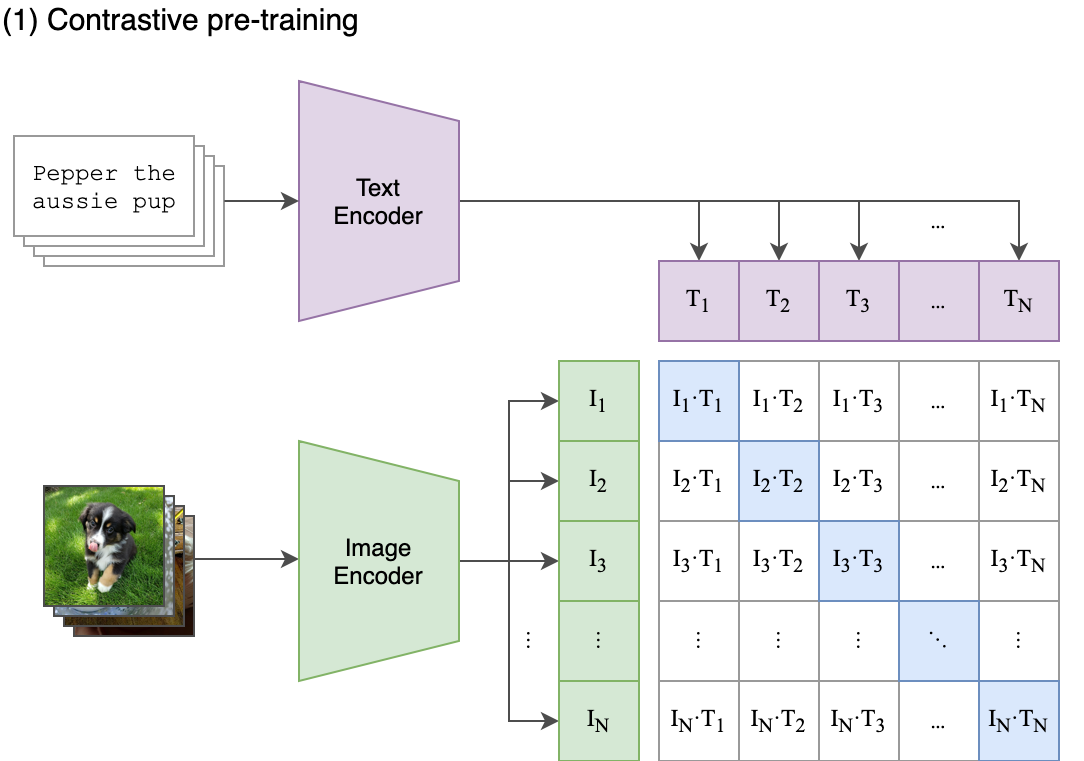
\includegraphics[width=0.7\linewidth]{modeling/CLIP.png}  
\caption{CLIP uses contrastive pre-training instead of generative objective to learn joint vision-language embeddings.}
\label{modeling.clip.pretrainingobj}
\end{figure*}

It is difficult to predict the exact captions for an image, since there is usually a wide variety of text descriptions co-occuring with images, so instead CLIP turns to contrastive objectives and solves the problem of determining which text and image should be matched together. 
As shown in Figure \ref{modeling.clip.pretrainingobj}, during pre-training, for a batch of $N$ (text,image) pairs, CLIP obtains $N$ image features and $N$ text features from the encoders. It then calculates the cosine similarities between each of the $N \times N$ pairings of the image and text features. The values are used as logit scores for calculating symmetric cross-entropy loss used to train the network.      


CLIP is trained on 400 million (image, text) pairs collected form a variety of publicly available sources on the Internet.

The query list that is used to compile these (image,text) pairs is the union of (1) words that occur $\geq 100$ times in English Wikipedia; (2) names of Wikipedia articles whose search volume is above certain threshold; (2) high pointwise mutual information (PMI) bi-grams, and (4) $117,000$ WordNet synsets, or sets of cognitive synonyms. 

\subsection{Image Pre-Processing}
We use the data provided by SPG \citep{spg_paper}, which provides JSON files of the Quick,Draw! sketches in vector format: each sketch is composed of a sequence of $n$ strokes $S_i, i \in [n]$, and $S_i$ is a sequence of vectors $(\delta x,\delta y, p, l)$. $\delta x$ and $\delta y$ are changes in the $x,y$ coordinates with respect to the previous point; for the first point, it is with respect to $(25,25)$. All points are assumed to be drawn on a $256 \times 256$ canvas. $p=1$ if the point is the last point in the current stroke, and $p=0$ otherwise. The SPG dataset provides annotation for semantic segmentation of the sketches, so $l$ is a number representing the semantically meaningful object part.  

% We obtained the rendered sketches by using \texttt{Pycairo}, which is a Python module providing bindings for the cairo graphics library. We use a line width of $5$. After rendering, we manually examined the sketches and filter out face sketches that do not have a pair of eyes, a mouth and the face outline; we also filter out angel sketches that are incomplete or have all the parts merged together, possibly due to collection errors in SPG.   

\subsection{Text Pre-Processing}
We used the \texttt{spacy} package to preprocess the text. \texttt{spacy} provides trained natural language processing pipeline and includes models for, for example, token-to-vector and part-of-speech tagging. We use the \texttt{en\_core\_web\_sm} pipeline and its lemmatizer to reduce words to their basic forms. Moreover, we lower-case all words and remove punctuation, a list of which is provided by \texttt{Python} \texttt{string} package, \texttt{string.punctuation}. We also remove words like \textit{shaped}, \textit{sized}, \textit{and}, \textit{like}, since they act like stop words and do not provide additional visual descriptions of the sketches. Text descriptions are also tokenized by CLIP's tokenizer before passing into CLIP text encoder.     

\section{Loss Function}
During training, for a given batch size $b$, we have $b$ sketch-text pairs, $(s_k,t_k), k\in [b]$. We are essentially using classification over $b$ classes to finetune CLIP, using cross-entropy loss. With clip, we obtain image logits $X_v$ over the text descriptions and text logits $X_t$ over the sketches. The ground-truth, for both image and text, is 
$Y_v = Y_t = \begin{bmatrix}1 & 2 & \cdots & b \end{bmatrix}^T $ 

$$L(X_v, Y_v) = \dfrac{1}{b} \sum_{k=1}^b -\log\frac{\exp{{X_v}_{k,k}}}{ \sum_{c=1}^b \exp{{X_v}_{k,c}} } $$

And similarly defined for $(X_t, Y_t)$,
$$L(X_t, Y_t) = \dfrac{1}{b} \sum_{k=1}^b -\log\frac{\exp{{X_t}_{k,k}}}{ \sum_{c=1}^b \exp{{X_t}_{k,c}} } $$

The final loss is defined as:
$$L = \dfrac{1}{2} (L(X_v, Y_v) + L(X_t, Y_t))$$

\section{Data Augmentation}
As mentioned above, our dataset has a small number of sketches: 572 face sketches and 787 angel sketches.  